%%%%%%%%%%%%%%%%%%%%%%%%%%%%%%%%%%%%%%%%%%%%%%%%%%%%%%%%%%%%%%%%%%%%%%%%%%%%%%%%
%2345678901234567890123456789012345678901234567890123456789012345678901234567890
%        1         2         3         4         5         6         7         8

\documentclass[letterpaper, 12 pt, conference]{ieeeconf}  % Comment this line out
                                                          % if you need a4paper
%\documentclass[a4paper, 12pt, conference]{ieeeconf}      % Use this line for a4
                                                          % paper

\IEEEoverridecommandlockouts                              % This command is only
                                                          % needed if you want to
                                                          % use the \thanks command
\overrideIEEEmargins
% See the \addtolength command later in the file to balance the column lengths
% on the last page of the document

\usepackage{hyperref}
\usepackage[utf8]{inputenc}
\usepackage{enumerate}
\usepackage{natbib}
\usepackage{graphicx}
\usepackage[spanish]{babel}
\hypersetup{
    colorlinks=true,
    linkcolor=blue,
    filecolor=magenta,      
    urlcolor=cyan,
}

% The following packages can be found on http:\\www.ctan.org
%\usepackage{graphics} % for pdf, bitmapped graphics files
%\usepackage{epsfig} % for postscript graphics files
%\usepackage{mathptmx} % assumes new font selection scheme installed
%\usepackage{times} % assumes new font selection scheme installed
%\usepackage{amsmath} % assumes amsmath package installed
%\usepackage{amssymb}  % assumes amsmath package installed

\title{\LARGE \bf
Práctica 3: puente de Wheatstone
}

%\author{ \parbox{3 in}{\centering Narshion Ngao*
%         \thanks{*Use the $\backslash$thanks command to put information here}\\
%         Msc. Computer Systems - 2018\\
%         Jomo Kenyatta University of Agriculture \& Technology \\
%       
%}}

\author{Universidad de San Carlos de Guatemala \\% <-this % stops a space
Escuela de Ciencias Físicas y Matemáticas\\
Laboratorio de Circuitos\\
Segundo Semestre 2019
}


\begin{document}



\maketitle
\thispagestyle{empty}
\pagestyle{empty}

\section{Objetivos}
\begin{itemize}
    \item General: poner en práctica los conocimientos adquiridos acerca del puente de Wheatstone y sus ecuaciones de análisis.
    \item Específicos:
    \begin{enumerate}
    \item Comprobar la eficiencia de la ecuación de diseño del puente de Wheatstone para estructuración de un circuito en equilibrio.
    \item Experimentar los cambios en el voltaje de salida del circuito en función de las variaciones en resistencia de un sensor (y las variables físicas asociadas).
\end{enumerate}
\end{itemize}


\section{Materiales}
\begin{itemize}
    \item 1 multímetro.
    \item 4 resistencias 1K ohm 1/4W.
    \item 2 resistencias 2K ohm 1/4W.
    \item 2 resistencias 3K ohm 1/4W.
    \item 1 potenciómetro de 1 Mohm.
    \item 1 fotorresistencia.
    \item 1 trozo pequeño de cinta de aislar.
    \item 1 trozo pequeño de cartón (suficiente para cubrir la fotorresistencia).
    \item Alambres para protoboard de cualquier tipo (y pinzas para cortarlo, si es necesario).
    \item 1 fuente.
    \item 1 protoboard.
    \item Opcional: computadora.
\end{itemize}
\pagebreak

\section{Diagramas}

\begin{figure}[h!]
    \centering
    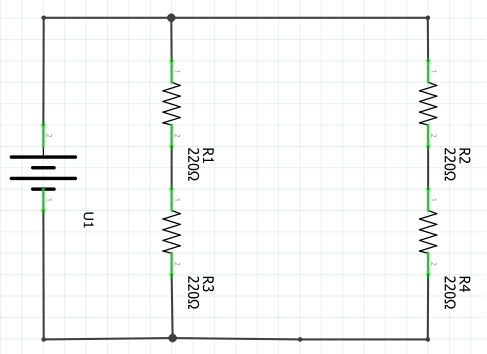
\includegraphics[scale=0.5]{C1.png}
    \caption{Esquema puente de Wheatstone con resistencias fijas.}
\end{figure}

\begin{figure}[h!]
    \centering
    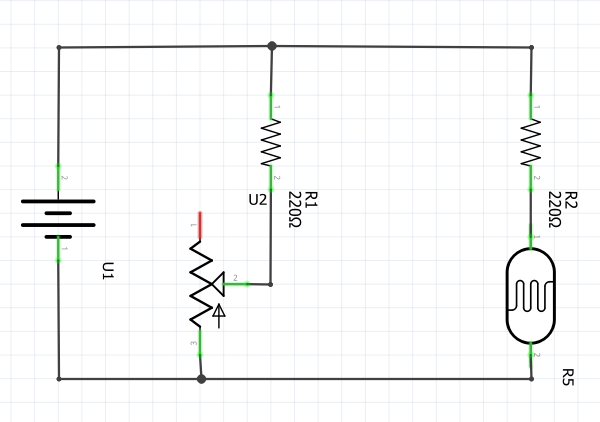
\includegraphics[scale=0.5]{C2.png}
    \caption{Esquema puente de Wheatstone con LDR.}
\end{figure}

\section{Procedimiento y reporte de resultados}
Seguir todos los pasos que a continuación se enlistan respondiendo en una hoja adicional lo que sea requerido de forma ORDENADA y CLARA.

\begin{enumerate}
    \item Utilizando la ecuación de diseño del puente de Wheatstone, encontrar los valores teóricos de voltaje de salida con R$_{2}/$R$_{1}$ en las cinco proporciones siguientes:
    \begin{itemize}
        \item 0.5
        \item 1
        \item 1.5
        \item 2
        \item 3
    \end{itemize}
    \item Armar en un protoboard el circuito de la Figura 1.

\begin{figure}[h!]
    \centering
    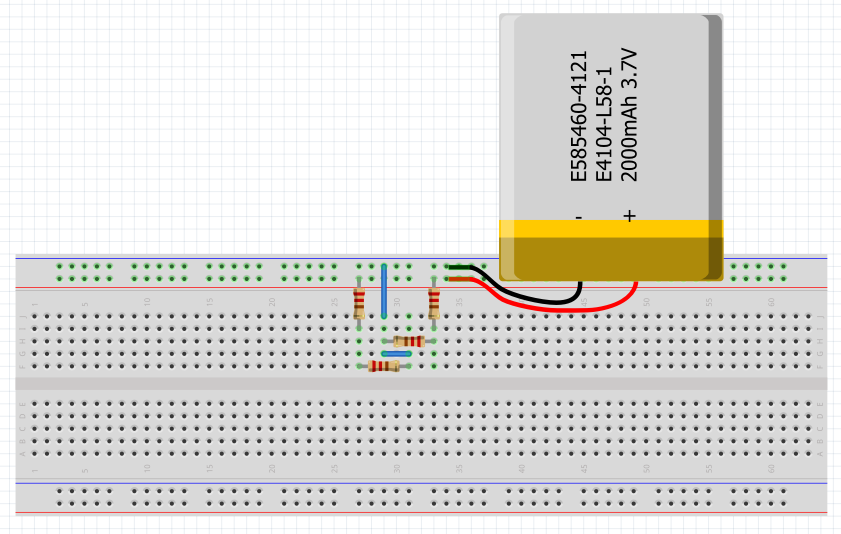
\includegraphics[scale=0.4]{B1.png}
    \caption{Circuito de Figura 1 en protoboard.}
\end{figure}
    \item Cambiar los valores de las resistencias que conforman el puente para ajustar las cinco combinaciones del inciso anterior. Medir para cada una el voltaje de salida.
    \item Realizar diagramas de incertezas para la comparación de valores obtenidos.
    \item Armar en un protoboard el circuito de la Figura 2.

\begin{figure}[h!]
    \centering
    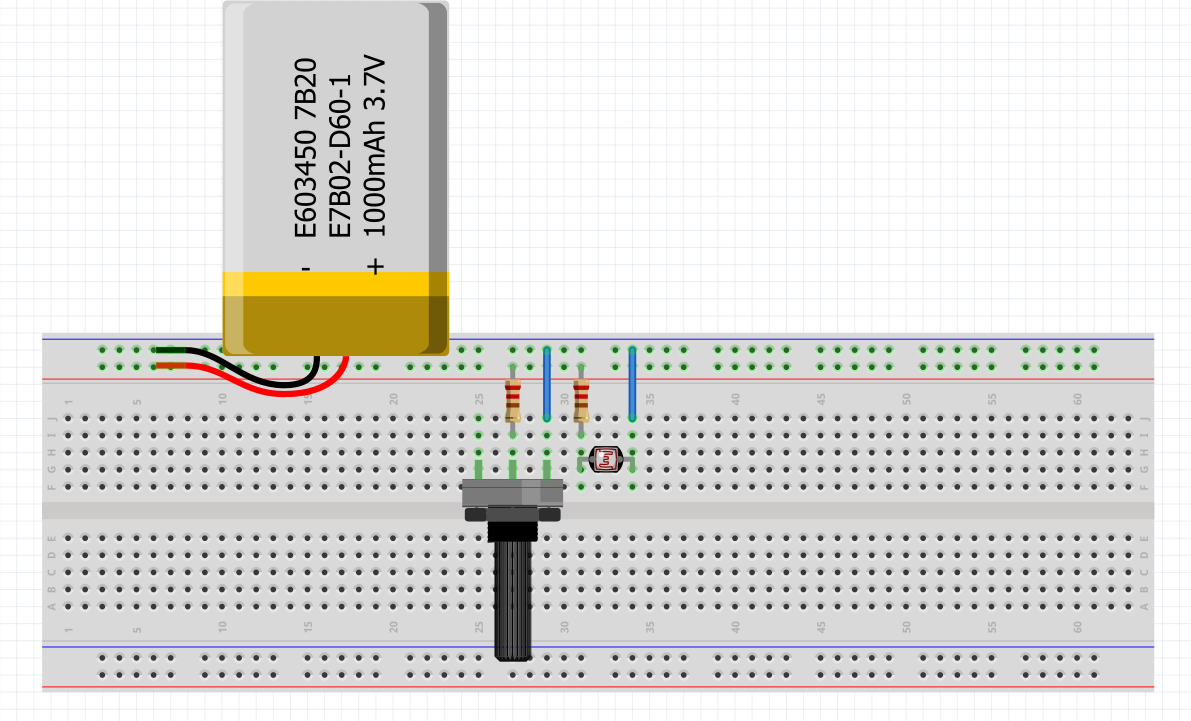
\includegraphics[scale=0.4]{B2.png}
    \caption{Circuito de Figura 2 en protoboard.}
\end{figure}
    \item Cubrir la fotorresistencia con un pedazo de cartón.
    \item Ubicar el multímetro en la salida del circuito para observar el voltaje, deberá variarse el potenciómetro hasta que la lectura de salida sea 0V.
    \item Cuando la condición sea alcanzada, medir la resistencia del potenciómetro y la de la LDR.
    \item Comprobar que los valores de resistencias cumplan las proporciones indicadas por las ecuaciones de diseño del circuito para puente en equilibrio.
    \item Repetir los últimos tres pasos otras dos veces con niveles distintos de iluminación.
    \item Contestar: según lo observado con el segundo circuito, ¿qué uso se podría dar a un puente de Wheatstone con LDR?
    \item Escribir las conclusiones de la práctica.
    
    
\end{enumerate}
\addtolength{\textheight}{-12cm}   % This command serves to balance the column lengths
                                  % on the last page of the document manually. It shortens
                                  % the textheight of the last page by a suitable amount.
                                  % This command does not take effect until the next page
                                  % so it should come on the page before the last. Make
                                  % sure that you do not shorten the textheight too much.

\end{document}